\documentclass[12pt]{article}

% math packages
\usepackage{amsmath, amsthm, amssymb, amsfonts}

% graphics packages
\usepackage{graphicx}

% code packages
\usepackage{listings}

% language packages
\usepackage[italian]{babel}

% page geometry
\usepackage[a4paper, portrait, margin=0.85in]{geometry}

% links
\usepackage[colorlinks]{hyperref}

% per le tabelle
\usepackage{adjustbox}

\newtheorem{definition}{Definizione}[section]

\newtheorem{theorem}{Teorema}[section]



\begin{document}

\title{
	Fondamenti di controlli automatici
}
\author{Ollari Ischimji Dmitri}

\maketitle

\newpage

\tableofcontents
\listoffigures
\listoftables


\section{Il controllo attivo di un processo}

Il \textbf{controllo attivo di un processo} permette la gestione dei processi, macchine e impianti riducendo l'intervento umano.

I principi del controllo attivo si basano sull'azione diretta (\textbf{feedforward}) e sull'azione di retroazione (\textbf{feedback}).

Il controllo attivo elimina il problema di imporre un funzionamento desiderato ad un processo.

La variabile controllata del sistema deve essere uguale al segnale di riferimento(che noi desideriamo).

\subsection{Sistema}
Un \textbf{sistema} è un complesso in cui si distinguono grandezze variabili nel tempo.

Le funzioni che rappresentano l'andamento delle variabili nel tempo prendono il nome di \textbf{segnali}.


Il \textbf{modello matematico(m.m.)} di un sistema è la descrizone del sistema in termini matematici, permettendo di identificare ingressi, uscite e disturbi.


Un sistema è \textbf{statico} se l'uscita dipende esclusivamente dall'ingresso nello stesso instante $t$, senza considerare tutti gli istanti precedenti:
\begin{align}
	\exists \quad f: \mathbb{R} \rightarrow \mathbb{R} \ni y(t) = f(u(t)) \forall t \in \mathbb{R}
\end{align}


Mentre un sistema \textbf{dinamico} prende in considerazione tutti gli istanti precendenti $t$ nell'intervallo di tempo $(-\infty, t]$:

\begin{align}
	\exists \quad F: K \rightarrow J \ni y(t) = F(u(\cdot)|_{(-\infty, t]}) \forall t \in \mathbb{R}
\end{align}

I sistemi dinamici introducono un concetto di sistema in \textbf{quiete}, \textbf{condizioni asintotiche} e \textbf{a regime}.


Generalemnte si rappresentano tutte le possibili coppie causa effetto mediante l'utilizzo dei \textbf{behaviors($\mathbf{B}$)}:
\begin{align}
	\mathbf{B} = \{ (u(t), y(t)) : y(t) \text{ uscita per ingresso } u(t), \quad t \in (-\infty, +\infty)\}
\end{align}

Un sistema si dice \textbf{lineare} quando soddisfa la proprietà di \textbf{sovrapposizione degli effetti}:
\begin{align}
	 & \forall (u_1, y_1), (u_2, y_2) \in \mathbf{B},                                                                                                                            \\
	 & \forall \alpha_1, \alpha_2 \in \mathbb{R} \Rightarrow \alpha_1(u_1, y_1) + \alpha_2(u_2, y_2) = (\alpha_1 u_1 + \alpha_2 u_2, \alpha_1 y_1 + \alpha_2 y_2) \in \mathbf{B}
\end{align}

Introduco anche la \textbf{stazionarieà} come l'invarianza nel tempo, se applico un'ingresso ora o lo applico fra 1 giorno, avro la stessa uscita.

\subsection{Feedforward}
L'azione di comando dipende da:
\begin{itemize}
	\item obiettivo perseguito
	\item informazioni sul modello del sistema
	\item disturbi
\end{itemize}

\begin{figure}[!ht]
	\centering
	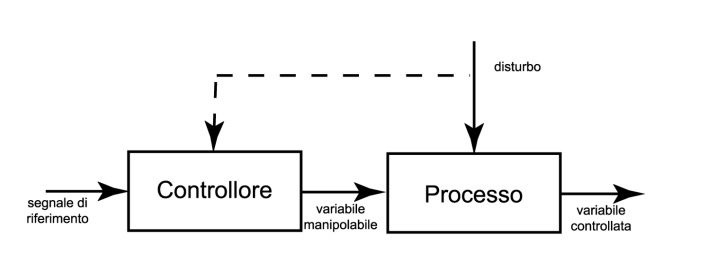
\includegraphics[width=0.5\textwidth]{./images/feedforward.png}
	\caption{Schema a blocchi di un sistema con feedforward}
	\label{fig:feedforward}
\end{figure}

\subsection{Feedback}

L'azione di comando dipende da:
\begin{itemize}
	\item obiettivo perseguito
	\item informazioni sul modello del sistema
	\item disturbi
	\item variabili controllate
\end{itemize}

\begin{figure}[!ht]
	\centering
	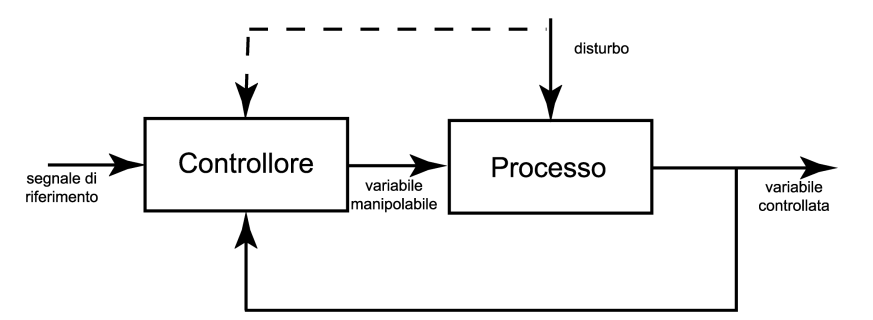
\includegraphics[width=0.5\textwidth]{./images/feedback.png}
	\caption{Schema a blocchi di un sistema con feedback}
	\label{fig:feedback}
\end{figure}


\subsection{Controllo diretto VS Controllo retroazionato}

L'errore in controllo diretto è $\pm 20 \%$ dove nel controllo in retroazione l'errore di inseguimento è circa $0.5\%$.

Il controllo in retroazione è efficace anche in presenza di perturbazioni sul processo. Parimenti, si potrebbe dimostrare che il controllo in retroazione è efficace anche in presenza di disturbi agenti sulla variabile controllata.



\section{Modellistica ed equazioni differenziali lineari}
% TODO:
% • Cenni di modellistica (circuiti elettrici e sistemi
% meccanici)
% • L’equazione differenziale lineare a coefficienti
% costanti quale modello di un sistema dinamico
% scalare



\subsection{Cenni di modellistica}

La modellistica è la costruzione di modelli matematici dei sistemi a partire dalle leggi fondamentali o dai dati sperimentiali.

\subsubsection{Circuiti elettrici - Resistenza}

\begin{figure}[!ht]
	\centering
	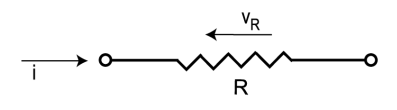
\includegraphics[width=0.3\columnwidth]{./images/resistenza.png}
	\caption{Resistenza}
	\label{fig:resistenza}
\end{figure}

\begin{align}
	V_R = R \cdot I
\end{align}


\subsubsection{Circuiti elettrici - Induttanza}

\begin{figure}[!ht]
	\centering
	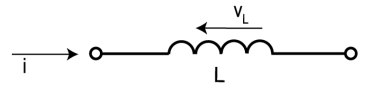
\includegraphics[width=0.3\columnwidth]{./images/induttanza.png}
	\caption{Induttanza}
	\label{fig:induttanza}
\end{figure}

\begin{align}
	V_L = L \cdot \frac{dI}{dt} = L \cdot DI
\end{align}


\subsubsection{Circuiti elettrici - Capacità}

\begin{figure}[!ht]
	\centering
	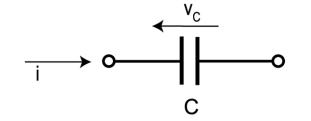
\includegraphics[width=0.3\columnwidth]{./images/capacita.png}
	\caption{Capacità}
	\label{fig:capacita}
\end{figure}

\begin{align}
	V_C = \frac{Q}{C} = \frac{1}{C} \int_{-\infty}^{t} i(\tau) d\tau \Rightarrow DV_C = \frac{I}{C}
\end{align}

\subsubsection{Sistemi meccanici - Massa}
\begin{figure}[!ht]
	\centering
	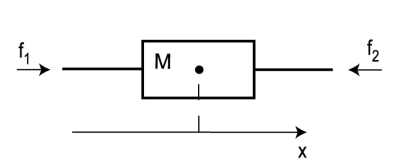
\includegraphics[width=0.3\columnwidth]{./images/massa.png}
	\caption{Massa}
  \label{fig:massa}
\end{figure}

\begin{align}
	MD^2 x(t) = f_1(t) - f_2(t)
\end{align}

\subsubsection{Sistemi meccanici - Molla}
\begin{figure}[!ht]
	\centering
	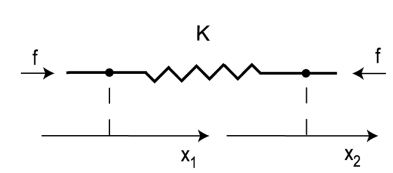
\includegraphics[width=0.3\columnwidth]{./images/molla.png}
	\caption{Molla}
  \label{fig:molla}
\end{figure}

\begin{align}
	f(t) = K(x_1(t) - x_2(t))
\end{align}


\subsubsection{Sistemi meccanici - Ammortizzatore}
\begin{figure}[!ht]
	\centering
	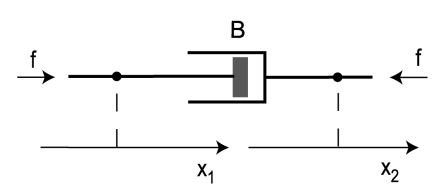
\includegraphics[width=0.3\columnwidth]{./images/ammortizzatore.png}
	\caption{Ammortizzatore}
	  \label{fig:ammortizzatore}
\end{figure}

\begin{align}
	f(t) &= B(v_1(t) - v_2(t)) \\
  &= BD(x_1(t) - x_2(t))
\end{align}




\subsection{Equazioni differenziali lineari}
Avendo un sistema di equazioni differenziali lineari a coefficienti costanti:
\begin{align}
  \sum_{i=0}^{n} a_i D^i y = \sum_{i=0}^{m} b_i D^i u
\end{align}


Si noti che:
\begin{itemize}
  \item $n$ è l'ordine dell'equazione differenziale se $n \geq m$
  \item $\rho = n - m$ è l'ordine relativo del sistema se $n \geq m$
\end{itemize}

\subsubsection{Proprietà}

Il sistema $\sum$ è lineare e stazionario.



\section{Cenni di analisi complessa}

\subsection{Poli}
Avendo la funzione:
\begin{align}
	f(s) = \frac{s(s+6)^3}{(s-2)(s+3)^2(s+5)^4}
  \label{eq:funzione_esempio_poli_e_zeri}
\end{align}

I poli sono quei valori di $s$ per i quali il denominatore si annulla, quindi:
\begin{itemize}
  \item $s = 2$ è un polo semplice
  \item $s = -3$ è un polo doppio
  \item $s = -5$ è un polo quadruplo
\end{itemize}

\subsection{Zeri}
Usando la funzione della \autoref{eq:funzione_esempio_poli_e_zeri}, gli zeri sono quei valori di $s$ per i quali il numeratore si annulla, quindi:
\begin{itemize}
  \item $s = 0$ è uno zero semplice
  \item $s = -6$ è uno zero triplo
\end{itemize}





\section{La trasformata di Laplace}

La trasformata di Laplace è un'operazione funzionale che converte una equazione differenziale in una equazione algebrica.

La trasfomata di Laplace di una funzione $f(t)$ è definita come:
\begin{align}
	F(s) = \int_{0}^{\infty} f(t) e^{-st} dt
\end{align}

\subsection{Transfomate di Laplace notevoli}
\renewcommand{\arraystretch}{2.0}
\begin{table}[!ht]
	\begin{adjustbox}{width=0.8\columnwidth,center}
		\begin{tabular}{|c|c|c|}
			\hline
			Segnale                               & $f(t)$                      & $F(s)$                                           \\
			\hline
			Gradino unitario                      & $1(t)$                      & $\frac{1}{s}$                                    \\
      \hline 
      Rampa unitaria                        & $t \cdot 1(t)$              & $\frac{1}{s^2}$                                  \\
      \hline
      Parabola unitaria                     & $\frac{1}{2}t^2 \cdot 1(t)$            & $\frac{1}{s^3}$                                  \\
			\hline
			Segnale esponeziale                   & $e^{at}$                    & $\frac{1}{s-a}$                                  \\
			\hline
			Derivata prima                        & $Df(t)$                     & $s F(s) - f(0)$                                  \\
			\hline
			Derivata di ordine $i$                & $D^i f(t)$                  & $s^i F(s) - \sum_{j=0}^{i-1} s^j D^{i-j-1} f(0)$ \\
			\hline
			Integrale                             & $\int_0^t f(x) dx$          & $\frac{1}{s} F(s)$                               \\
			\hline
			Traslazione nel tempo                 & $f(t - t_0) \cdot 1(t-t_0)$ & $e^{-t_0 s} F(s)$                                \\
			\hline
			Traslazione nella variabile complessa & $e^{at} f(t)$               & $F(s-a)$                                         \\
			\hline
			-                                     & $t^n e^{at}$                & $\frac{n!}{(s-a)^{n+1}}$                         \\
			\hline
			Convoluzione                          & $\int_0^t f(x)g(t-x)dx$     & $F(s)G(s)$                                       \\
			\hline
		\end{tabular}
	\end{adjustbox}
	\caption{Trasformate di Laplace}
	\label{tab:laplace}
\end{table}

\subsection{Proprietà della trasformata di Laplace}
La linearità della trasformata di Laplace è definita come:
\begin{align}
	\mathcal{L} [a f(t) + b g(t)] = a \mathcal{L} [f(t)] + b \mathcal{L} [g(t)]
\end{align}

Mentre l'iniettività è definita come:
\begin{align}
	\mathcal{L} [f(t)] = \mathcal{L} [g(t)] \implies f(t) = g(t)
\end{align}


\subsection{Anti-trasformata di Laplace}

Sia:
\begin{align}
	F(s) = \frac{b(s)}{a(s)}
\end{align}

Assumneto che:
\begin{itemize}
	\item $\deg b(s) < \deg a(s)$
	\item $a(s)$ e $b(s)$ sono coprimi fra loro
	\item $n := \deg a(s)$
	\item Poli semplici
\end{itemize}

Posso definire la anti-trasformata di Laplace come:
\begin{align}
	f(t) = \mathcal{L}^{-1} [F(s)]
\end{align}


Per ricondurre la formula in somma si poli semplici si ricorre allo \textbf{sviluppo in fratti semplici} per ricondurre la formula a:
\begin{align}
	F(s) = \frac{k_1}{s-p_1} + \frac{k_2}{s-p_2} + \dots + \frac{k_n}{s-p_n}
\end{align}

Dove $k_i$ sono i residui e $p_i$ sono i poli.

Per calcolare i residui si usa la formula:
\begin{align}
	k_i = (s - p_i) F(s) \bigg|_{s = p_i} \quad i = 1, \dots, n
\end{align}

Il che ci porta ad avere una formula per l'antitraformata di Laplace:
\begin{align}
	f(t) = \sum_{i=1}^{n} k_i e^{p_i t}
\end{align}



\section{Le funzioni impulsive e l'insieme dei behaviors}

\subsection{Le funzioni impulsive}

Gradino unitario:
\begin{align}
	1(t) := \begin{cases}
		        0 & t < 0    \\
		        1 & t \geq 0
	        \end{cases}
\end{align}

Introduco la funzione $f(t;\tau) \in \mathcal{C}^0$:
\begin{align}
	f(t;\tau) := \begin{cases}
		             0               & t < \tau        \\
		             \frac{1}{\tau}t & 0 \leq t < \tau \\
		             1               & t > \tau
	             \end{cases}
\end{align}

Formalmente si definisce la \textbf{delta di Dirac} come:
\begin{align}
	\delta(t) := \lim_{\tau \to 0} Df(t;\tau)
\end{align}

Ricordo che la derivata di una funzione $f(t:\tau)$ è:

\begin{align}
	Df(t;\tau) := \begin{cases}
		              0              & t < \tau        \\
		              \frac{1}{\tau} & 0 \leq t < \tau \\
		              1              & t > \tau
	              \end{cases}
\end{align}


\subsection{Derivata generalizzata di una funzione discontinua}

$f \in \mathcal{C}^{+\infty}_p(\mathbb{R})$ e sia $t = 0$ il solo istante di discontionuità di $f$.

Definisco la derivata generalizzata di $f$ come:
\begin{align}
	g(t) & := \begin{cases}
		          f(t)               & t < 0    \\
		          f(t) - (f_+ - f_-) & t \geq 0 \\
	          \end{cases} \\
	g(t) & \in \mathcal{C}^0
\end{align}


Ovvero che la \textbf{funzione discontinua} $=$ \textbf{funzione continua} $+$ \textbf{funzione a gradino}.

Usando la derivata generalizzata:
\textbf{Derivata generalizzata di ordine 1} $=$ \textbf{funzione discontinua} $+$ \textbf{funzione impulsiva(ordine 0)}.



Principio di identità delle funzioni impulsive:
Le funzione impulsiva:
\begin{align}
  c_{-1} + c_0\delta(0) + c_1\delta'(0) + c_2\delta''(0) + \dots + c_n\delta^{(n)}(0)
\end{align}

E la funzione impulsiva:
\begin{align}
  d_{-1} + d_0\delta(0) + d_1\delta'(0) + d_2\delta''(0) + \dots + d_m\delta^{(m)}(0)
\end{align}

Sono uguale se e solo se:
\begin{align}
  c_i = d_i \quad \forall i = 0, 1, \dots, \min \{ n, m \}
\end{align}

Se $n > m$ allora $c_i = 0, i = m + 1, \dots, n$, altrimenti \\
se $m > n$ allora $d_i = 0, i = n + 1, \dots, m$.

\section{La funzione di trasferimento}
\subsection{Estensione dell'insieme dei behaviors}

Dato un sistema dinamico $\sum$ descritto dall'equazione differenziale:
\begin{align}
  \sum_{i=0}^n a_i D^i y = \sum_{i=0}^m b_i D^i u
\end{align}

Si definisce estensione impulsiva dei behaviors o \textbf{behavior esteso} di $\sum$:
\begin{align}
  \mathcal{B}^* := \{ (u, y) \in \mathcal{C}_p^{\infty} (\mathbb{R})^* \times \mathcal{C}_p^{\infty} (\mathbb{R})^* : \sum_{i=0}^n a_i D^{*i} y = \sum_{i=0}^m b_i D^{*i} u \}
\end{align}

\begin{align}
  \mathcal{B} \subset \mathcal{B}^*
\end{align}

Se ne ricava una proprietà importante:
\begin{align}
  (u, y) \in \mathcal{B}^* \Rightarrow (D^* u, D^*y) \in \mathcal{B^*}
\end{align}


\subsection{Problema fondamentale dell'analisi nel dominio del tempo di un sistema $\sum$}

Avendo l'equazione differenziale che descrive il sistema $\sum$:
\begin{align}
  \sum_{i=0}^n a_i D^{*i} y(t) = \sum_{i=0}^m b_i D^{*i} u(t)
\end{align}

\textbf{Si deve applicare la trasformata di Laplace}:
\begin{align}
  \sum_{i=0}^n a_i \mathcal{L}[  D^{*i} y(t) ] &= \sum_{i=0}^m b_i \mathcal{L}[ D^{*i} u(t) ] \\
  \sum_{i=0}^n a_i s^i Y(s) &= \sum_{i=0}^m b_i s^i U(s)
\end{align}

Si definisce funzione di trasferimento del sistema $\sum$:
\begin{align}
  G(s) := \frac{Y(s)}{U(s)} = \frac{\sum_{i=0}^m b_i s^i}{\sum_{i=0}^n a_i s^i}
  \label{eq:funzione_trasferimento}
\end{align}



\subsubsection{Sistema proprio} % (fold)
\label{sec:Sistema proprio}
Un sistema si dice \textbf{(strettamente)proprio} se la sua funzione di trasfermento è una funzione razionale (strettamente)propria, cioè:
\begin{itemize}
  \item $n \geq m \implies \rho \geq 0$ il sistema è proprio
  \item $n > m \implies \rho \geq 1$ il sistema è strettamente proprio
\end{itemize}
% subsubsection Sistema proprio (end)


\subsubsection{Guadagno statico} % (fold)
\label{sec:Guadagno statico}

Rapporto fra valore costante dell'uscita e il valore costante dell'ingresso:
\begin{align}
  K := \frac{y_c}{u_c}
\end{align}

% subsubsection Guadagno statico (end)

\subsubsection{Polinomio caratteristico} % (fold)
\label{sec:Polinomio caratteristico}

Dato il sistema $\sum$:
\begin{align}
  \sum_{i=0}^n a_i D^{i} y = \sum_{i=0}^m b_i D^{i} u
\end{align}

Il polinomio caratteristico è:
\begin{align}
  a(s) := \sum_{i=0}^n a_i s^i
\end{align}

% subsubsection Polinomio caratteristico (end)

\subsubsection{Poli e Zeri} % (fold)
\label{sec:Poli e Zeri}
Avendo una funzione di trasferimento $G(s)$:
\begin{align}
  G(s) = \frac{b(s)}{a(s)}
\end{align}

gli zeri sono i valori di $s$ che annullano il numeratore $b(s)$, i poli sono i valori di $s$ che annullano il denominatore $a(s)$.
% subsubsection Poli e Zeri (end)

\subsubsection{Modi} % (fold)
\label{sec:Modi}
Se $p$ è un polo \textbf{reale} con molteplicità $h$:
\begin{align}
  e^{pt}, te^{pt}, \dots, t^{h-1}e^{pt}
\end{align}

Se $\sigma \pm j \omega$ è un polo \textbf{complesso} coniugato con molteplicità $h$:
\begin{align}
  e^{\sigma t} \sin(\omega t + \phi_1), te^{\sigma t} \sin(\omega t + \phi_2), \dots, t^{h-1}e^{\sigma t} \sin(\omega t + \phi_h)
\end{align}

oppure:
\begin{align}
  e^{\sigma t} \sin(\omega t), e^{\sigma t} \cos(\omega t), \dots, t^{h-1}e^{\sigma t} \sin(\omega t), t^{h-1}e^{\sigma t} \cos(\omega t)
\end{align}
% subsubsection Modi (end)


\subsubsection{Risposte canoniche} % (fold)
\label{sec:Risposte canoniche}
Usualmente le risposte canocniche prese in considerazione sono:
\begin{itemize}
  \item $g(t) \equiv$ risposta all'impulso $\delta(t)$
  \item $g_s(t) \equiv$ risposta al gradino $1(t)$
\end{itemize}
% subsubsection Risposte canoniche (end)

\section{Sistemi dinamici elementari} % (fold)
\label{sec:Sistemi dinamici elementari}

% section Sistemi dinamici elementari (end)

\section{La stabilità dei sistemi dinamici}

\subsection{Definizioni e teoremi}

Considerando il sistema dinamico seguente:
\begin{align}
    \sum_{i=0}^{n} a_i D^i y = \sum_{i=0}^{m} b_i D^i u
\end{align}

La funzione di trasferimento è:
\begin{align}
    G(s) = \frac{b}{a}
\end{align}


Il guadagno statico è definito dal valore per $s=0$:
\begin{align}
    G(0) = \frac{b_0}{a_0}
\end{align}

% \begin{definition}[Perturbazione dell'evoluzione]
%     Data la coppia $(u(t), y(t)) \in \mathcal{B}$, una perturbazione di questa è caratterizzata
%     da una modifica nell'intervallo $[t_0, 0)$ sia dall'ingresso sia dall'uscita determinando la coppia 
%     perturbata $(\hat{u(t)}, \hat{y(t)}) \in \mathcal{B}$
% \end{definition}

\begin{definition}[stabilità (alle perturbazioni) di un sistema dinamico lineare]
    Il sistema si dice:
    \begin{itemize}
        \item \textbf{Stabile} se per ogni perturbazione la risposta libera è limitata su $[0, +\infty[$
        \item \textbf{Asintoticamente stabile} se è stabile e inoltre la risposta libera tende a zero per tempi infiniti
        \item \textbf{Semplicemente stabile} se è stabile e inoltre esiste una perturbazione per la quale la risposta libera non è limitata
        \item \textbf{Instabile} se non è stabile 
    \end{itemize}
\end{definition}


\begin{theorem}[Poli e stabilità]
    Sia un sistema lineare per il quale i poli coincidono con le radici del polinomio caratteristico
    ($a(s)$ e $b(s)$ sono coprimi fra loro), allora: 
    \begin{itemize}
        \item Il sistema è \textbf{stabile} se e solo se tutti i poli hanno parte reale non positiva e gli eventuali poli puramente immaginari sono semplici
        \item Il sistema è \textbf{asintoticamente stabile} se e solo se tutti i suoi poli hanno parte reale negativa
        \item Il sistema è \textbf{semplicemente stabile} se e sono se tutti i poli hanno parte reale non positiva e quelli puramente immaginari (che devono esistere) sono semplici
        \item Il sistema è \textbf{instabile} se e sono se esiste almeno un polo a parte reale positiva oppure un polo puramente immaginario con molteplicità maggiore di uno
    \end{itemize}
\end{theorem}


\subsection{Stabilità Bounded Input Bounded Output(BIBO)}

\begin{definition}[BIBO]
    Un sistema è BIBO stabile se per ogni azione forzante limitata la corrispondente
    risposta forzata è anch'essa limitata.
\end{definition}

\subsection{Criterio di Routh}
Considerando il sistema descritto dall'equazione differenziale:
\begin{align}
    \sum_{i=0}^{n}  a_i D^i y = \sum_{i=0}^{m}  b_i D^i u
\end{align}

\begin{definition}[Equazione caratteristica]
    Dato il sistema, l'equazione $a(s) = 0$ è detta equazione caratteristica del sistema.
\end{definition}

\begin{definition}[Polinomio di Hurwitz]
    Un polinomio $a(s)$ è detto di Hurwitz o hurwitziano se tutte le sue radici hanno parte reale negativa.
\end{definition}

È possibile determinare il segno delle radici di $a(s)$ mediante l'uso della \textbf{tabella di Routh}.

La tabella di Routh è una procedura algoritmica usata in controllo automatico per determinare la stabilità di un sistema dinamico lineare. Per un dato polinomio caratteristico, la tabella di Routh è costruita seguendo determinate regole per organizzare i coefficienti del polinomio. La stabilità del sistema è determinata dal segno dei coefficienti nella prima colonna della tabella: se tutti i coefficienti sono positivi, allora il sistema è stabile.

La base della tabella di Routh segue questo schema:
\begin{table}[h!]
    \centering
    \begin{tabular}{c | c c c c}
        $n$ & $x_{0, 0}$ & $x_{0, 1}$ & $x_{0, 2}$ & \dots \\
        $n-1$ & $x_{1, 0}$ & $x_{1, 1}$ & $x_{1, 2}$ & \dots \\
        $n-2$ & $x_{2, 0}$ & $x_{2, 1}$ & $x_{2, 2}$ & \dots \\
        \dotfill
    \end{tabular}
\end{table}

Le prime due righe della tabella di Routh sono i coefficienti di $a(s)$, ecco un esempio:
\begin{align}
    a_n s^n +
    a_{n-1} + s^{n-1} +
    a_{n-2} + s^{n-2} +
    a_{n-3} + s^{n-3} +
    a_{n-4} + s^{n-4} +
    a_{n-5} + s^{n-5} + 
    \dots
\end{align}

Vengono posizionati nelle prime due righe della tabella di Routh nel seguente modo:
\begin{table}[h!]
    \centering
    \begin{tabular}{c | c c c c}
        $n$ & $a_n$ & $a_{n-2}$ & $a_{n-4}$ & \dots \\
        $n-1$ & $a_{n-1}$ & $a_{n-3}$ & \dots & \dots
        \dotfill
    \end{tabular}
\end{table}
Mentre tutte le altre parti della tabella vengono calcolate come segue:
\begin{align}
    x_{i, j} &= - \frac{
        \begin{bmatrix}
            x_{i-2, 0} & x_{i-2, j+1} \\
            x_{i-1, 0} & x_{i-1, j+1}
        \end{bmatrix}
    }{x_{i-1, 0}} \\
    &= \frac{x_{i-1, 0} \cdot x_{i-2, j+1} - x_{i-2, 0} \cdot x_{i-1, j+1} }{x_{i-1, 0}}
\end{align}


\begin{definition}[Routh]
    Si assuma che la tabella di Routh possa essere completata.    
    Allora a ogni variazione di segno degli elementi della prima colonna,
    corrisponde a una radice con parte reale positiva.
\end{definition}

\begin{definition}[Criterio di Routh]
    Il polinomio $a(s)$ è hurwitziano se e solo se l'associata tabella di Routh
    può essere completata (con l'algoritmo di base) e presenta nella prima 
    colonna solo permanenze del segno.
\end{definition}

\subsection{Casi particolari nella costruzione della tabella di Routh}
Esistono due casistiche:
\begin{itemize}
    \item Primo elemento di una riga uguale a zero
    \item Tutti gli elementi di una riga uguali a zero
\end{itemize}


\subsubsection{Caso 1}
Si utilizza il metodo di \textbf{Benidir-Picinbono} che è sempre risolutivo.


\begin{theorem}[Metodo di Benidir-Picinbono]
    Ogni riga non nulla che inizia con $p$ zeri viene sommata con la riga da questa ottenuta
    moltiplicandola per $(-1)^p$ e traslandola verso sinistra di $p$ posizioni.
    La tabella di Routh viene poi continuata e interpretata nel modo usuale.
\end{theorem}


Segue un esempio:
\begin{align}
    a(s) = s^3 + 3s -2 = 0
\end{align}

\begin{table}[h!]
    \centering
    \begin{tabular}{c | c c c}
        $3$ & $1$ & $3$ & $0$ \\
        $2$ & $0$ & $-2$ & $0$ \\
    \end{tabular}
\end{table}

Visto che la riga numero due Inizia con $p=1$ zeri, allora devo sommare la riga due
con la riga due moltiplicata per $(-1)^1 = -1$ e traslata di uno posizione verso
sinistra:

\begin{table}[h!]
    \centering
    \begin{tabular}{c | c c c}
        $3$ & $1$ & $3$ & $0$ \\
        $2$ & $2$ & $-2$ & $0$ \\
    \end{tabular}
\end{table}

E poi si continua con il metodo di Routh tenendo in considerazione che 
il metodo procede come al solito.

\subsubsection{Caso 2}
Se tutti gli elementi di una riga sono uguali a zero, si deve definire un polinomio ausiliario
che prende la riva immediatamente precedente e si calcola la derivata di questo polinomio.


\section{Analisi armonica e diagrammi di Bode}

\subsection{L'analisi armonica nei sistemi lineari}

Considerando un sistema dinamico $\sum$, asintoticamente stabile, descritto come:
\begin{align}
    \sum_{i=0}^{n} a_i D^i y = \sum_{i=0}^{m} b_i D^i u
\end{align}

($a(s)$ e $b(s)$ sono coprimi fra loro), la funzione di trasferimento è:

\begin{figure}[h!]
    \centering
    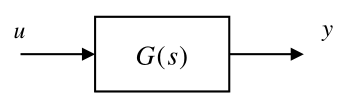
\includegraphics[width=0.3\textwidth]{images/fdt.png}
    \caption{Funzione di trasferimento}
    \label{fig:fdt}
\end{figure}

\begin{align}
    G(s) = \frac{b(s)}{a(s)}
\end{align}



\begin{theorem}
    Sia $\sum$ un sistema asintoticamente stabile con funzione di trasferimento $G(s)$
    razionale.
    La risposta forzata del sistema a un segnale armonico in ingresso è 
    a sua volta un segnale armonico con la stessa frequenza(per $t \to \infty$).
    \`E soddisfatta la relazione:
    \begin{align}
        F(\omega) = G(j\omega)
    \end{align}
\end{theorem}



\subsection{Guadagni del sistema lineare}
Avendo una funzione di trasferimento $G(s)$, si possono individuare i guadagni del sistema:
\begin{itemize}
    \item Guadagno statico: $G(0)$
    \item Guadagno armonico: $|G(j\omega)|$
\end{itemize}


\subsection{Diagrammi di Bode}
Il diagramma di Bode è un grafico che rappresenta il modulo e la fase della funzione di trasferimento
in funzione della pulsazione $\omega$.

Il modulo è rappresentato in scala logaritmica, mentre la fase è rappresentata in scala lineare.
Le varie rappresentazioni sono:
\begin{align}
    G(j\omega) &= | G(j\omega) | e^{j \angle G(j\omega)} \\
    &= | G(j\omega) | \angle G(j\omega)
\end{align}

Nello specifico, il modulo è rappresentato in decibel:
\begin{align}
    db = 20 \log_{10} | G(j\omega) |
\end{align}

Mentre la fase è rappresentata in gradi:
\begin{align}
    \angle G(j\omega) = \arg G(j\omega)
\end{align}


\subsection{Rappresentazioni e parametri della funzione di trasferimento}
Le rappresentazioni della funzione di trasferimento sono \textbf{forma standard con polinomi monici} e  
\textbf{forma standard con poli e zeri}.

La forma standard con polinomi monici è:
\begin{align}
    G(s) = \frac{b(s)}{a(s)} = K_1 \frac{s^m + b_{m-1} s^{m-1} + \dots + b_0}{s_n + a_{n-1} s^{n-1} + \dots + a_0}
\end{align}

Mentre la forma standard con poli e zeri è:
\begin{align}
    G(s) = \frac{b(s)}{a(s)} = K_1 \frac{(s - z_1)(s-z_2) \dots (s-z_m)}{(s-p_1)(s-p_2) \dots (s-p_n)}
\end{align}

In entrambe le forme, $K_1$ è la costante di trasferimento.


\subsection{Parametri caratteristici della risposta armonica}


\begin{table}[h!]
    \centering
    \begin{tabular}{| c | c |}
    \hline
        Pulsazione di risonanza & $\omega_R := \arg \max |G(j\omega)|$ \\
        Picco di risonanza & $M_R := \frac{|G(j\omega_R)|}{|G(j0)|}$ \\
        Larghezza di banda & $ B_{\omega} := \omega_{t2} - \omega_{t1} $ \\
    \hline
    \end{tabular}
\end{table}

$\omega_{t2} > \omega_{t1} \geq 0$ prendono il nome di pulsazioni di taglio e rispettivamente
sono la pulsazione di taglio superiore e quella inferiore.



\section{I diagrammi di Nyquist e i sistemi a fase minima}

\subsection{I diagrammi polari o di Nyquist}
I diagrammi polari o di Nyquist sono importanti nello studio della stabilità
dei sistemi retroazionati.

Prendendo come esempio la funzione di trasferimento:
\begin{align}
    G(j\omega) = \frac{10}{(1 + \frac{1}{5} j\omega)(1 + \frac{1}{10} j\omega)(1 + \frac{1}{100} j\omega)}
\end{align}



Si possono calcolare i punti del diagramma di Nyquist mediante l'utilizzo di 
modulo e fase della funzione di trasferimento:
\begin{align}
    |G(j\omega)| = K_1 \frac{M_1}{M_2 M_3 M_4}
\end{align}

\begin{align}
    \angle G(j\omega) = \begin{cases}
        \varphi_1 - \varphi_2 - \varphi_3 - \varphi_4 & \text{se } K_1 > 0 \\
        \varphi_1 - \varphi_2 - \varphi_3 - \varphi_4 - \pi & \text{se } K_1 < 0
    \end{cases}
\end{align}


\subsection{I sistemi a fase minima}

\begin{definition}[Sistemi a fase minima(non minima)]
    Sia $\sum$ un sistema lineare e stazionario con funzione di trasferimento
    $G(s)$ e risposta armonica $G(j\omega)$.
    
    $\sum$ si dice a fase minima (fase non minima) se il diagramma delle fasi
    $\beta = \arg G(j\omega)$ è (non è) determinata univocamente, con modulo $2\pi$,
    dal diagramma dei moduli $\alpha = |G(j\omega)|$ mediante la formula di Bode.
\end{definition}

Si ricava che una funzione di trasferimento \textbf{razionale} $G(s)$ è a fase
minima se e solo se non sono presenti poli o zeri con parte reale positiva.



\subsection{Approssimanti di Padé del ritardo finito}

L'Approssimante di Padé di $e^{-t_0 s}$ di ordine $q$ è la funzione razionale:
\begin{align}
    G_q (s; t_0) := \frac{
        \sum_{k=0}^q \frac{(2q - k)! q!}{(2q)!k!(q-k)!} (-1)^k t_0^k s^k
    }{
        \sum_{k=0}^q \frac{(2q - k)! q!}{(2q)!k!(q-k)!} t_0^k s^k
    }
\end{align}


\subsection{Tracciamento qualitativo del diagramma polare (o di Nyquist) della risposta armonica di un sistema $G(s)$}
\begin{enumerate}
    \item Scrivere $G(s)$ nella forma standard con le costanti di tempo
        \begin{itemize}
            \item Se non ci sono poli nell'origine ($h=0$), può andar bene la forma
                standard con i poli e gli zeri reali.
            \item Si sostituisce ad $s$ la variabile $j\omega$.
        \end{itemize}
    \item Si determinano le espressioni di $|G(j\omega)|$ e $\angle G(j\omega)$
        in funzione di $\omega$.
        
    \item Si studia il comportamento di $|G(j\omega)|$ e $\angle G(j\omega)$
        per $\omega \to 0$ e $\omega \to \infty$.
    
    \item Si determina l'intersezione del diagramma polare con l'asse reale negativo
        (se esiste).
        
    \item Sulla base dei punti precedenti si traccia il diagramma polare.
\end{enumerate}
\section{Sistemi retroazionati: proprietà e analisi asintotica}

\subsection{Schemi a blocchi}
I sistemi complessi possono essere rappresentati mediante l'uso di schemi
a blocchi, alcuni esempi dei blocchi pi\`u comuni:

\begin{figure}[h!]
    \centering
    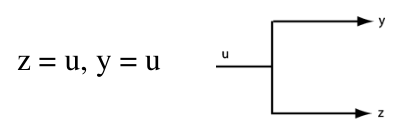
\includegraphics[width=0.3\linewidth]{images/blocchi_diramazione.png}
    \caption{Blocchi di diramazione}
    \label{fig:diramazione}
\end{figure}

\begin{figure}[h!]
    \centering
    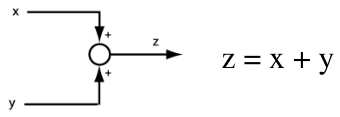
\includegraphics[width=0.3\linewidth]{images/blocchi_sommanti.png}
    \caption{Blocchi sommanti}
    \label{fig:sommanti}
\end{figure}


\subsection{Regole di riduzione}
\begin{figure}[h!]
    \centering
    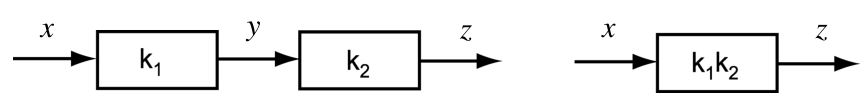
\includegraphics[width=0.3\linewidth]{images/riduzione_cascata.png}
    \caption{Riduzione di blocchi in cascata}
    \label{fig:cascata}
\end{figure}

\begin{figure}[h!]
    \centering
    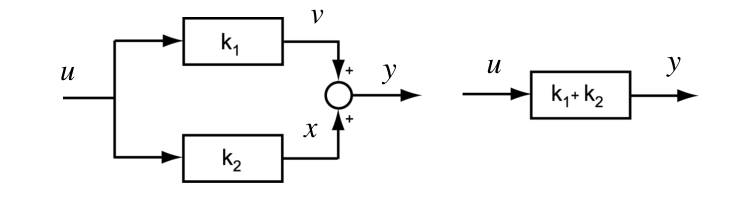
\includegraphics[width=0.3\linewidth]{images/riduzione_parallelo.png}
    \caption{Riduzione di blocchi in parallelo}
    \label{fig:parallelo}
\end{figure}


\begin{figure}[h!]
    \centering
    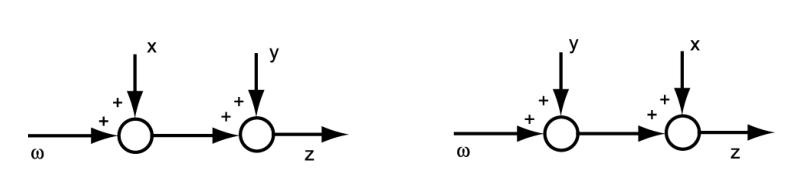
\includegraphics[width=0.3\linewidth]{images/scambio_giunzioni_sommanti.png}
    \caption{Scambio di giunzioni sommanti}
    \label{fig:scambio_sommanti}
\end{figure}


\begin{figure}[h!]
    \centering
    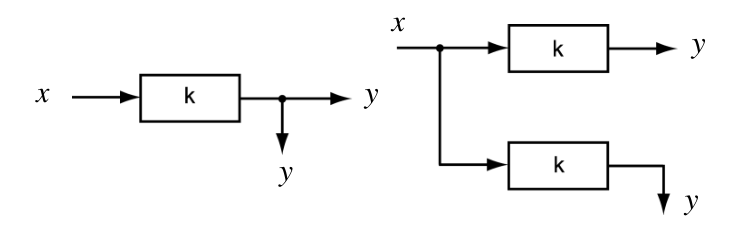
\includegraphics[width=0.3\linewidth]{images/spostamento_prelievo_segnale.png}
    \caption{Spostamento di prelievo di segnale a monte di un blocco}
    \label{fig:spostamento_prelievo_monte}
\end{figure}


\begin{figure}[h!]
    \centering
    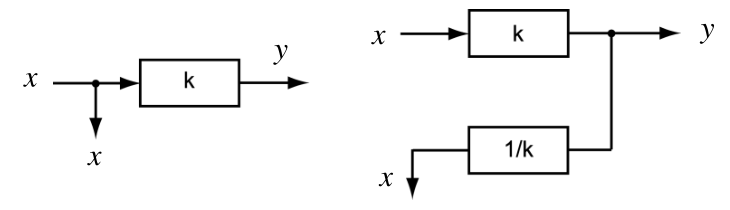
\includegraphics[width=0.3\linewidth]{images/spostamento_prelievo_segnale_a_valle.png}
    \caption{Spostamento di prelievo di un segnale a valle di un blocco}
    \label{fig:spostamento_prelievo_valle}
\end{figure}

\begin{figure}[h!]
  \centering
  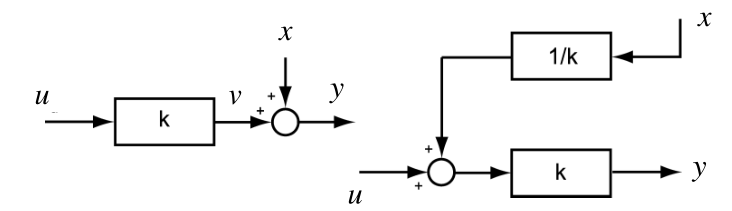
\includegraphics[width=0.3\linewidth]{images/spostamento_giunzione_a_monte.png}
  \caption{Spostamento di giunzione sommante a monte di un blocco}
  \label{fig:spostamento_giunzione_monte}
\end{figure}



\begin{figure}[h!]
  \centering
  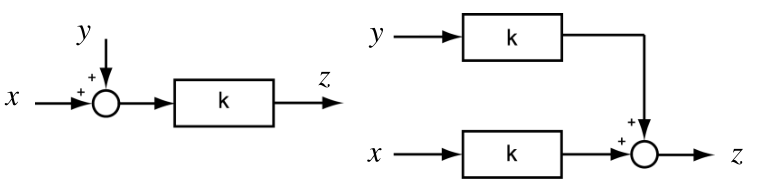
\includegraphics[width=0.3\linewidth]{images/spostamento_giunzione_a_valle.png}
  \caption{Spostamento di giunzione sommante a valle di un blocco}
  \label{fig:spostamento_giunzione_valle}
\end{figure}


\begin{figure}[h!]
  \centering
  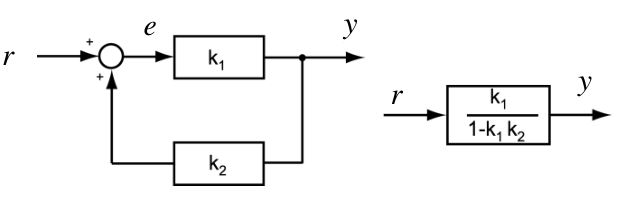
\includegraphics[width=0.3\linewidth]{images/eliminazione_anello.png}
  \caption{Eliminazione di un anello}
  \label{fig:eliminazione_anello}
\end{figure}



\newpage
\subsection{Proprietà generali dei sistemi in retroazione}
\begin{figure}[h!]
  \centering
  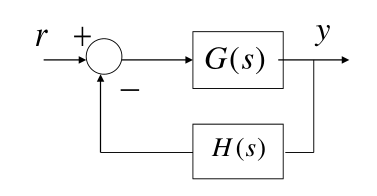
\includegraphics[width=0.3\linewidth]{images/retroazione.png}
  \caption{Schema a blocchi di un sistema in retroazione}
  \label{fig:retroazione}
\end{figure}


La funzione di trasferimento risulta:
\begin{align}
  \text{FDT} &= \frac{\text{fdt del percorso diretto}}{1 + \text{guadagno ad anello}} \\
  &= \frac{G(s)}{1 + G(s)H(s)}
\end{align}

Osservazioni:
\begin{itemize}
  \item Un guadagno di anello elevato rende (relativamente) 
        insensibile la f.d.t. del sistema retroazionato a variazioni della 
        f.d.t. del sistema controllato
  \item Variazioni della f.d.t. nella catena di retroazione si 
        riverberano senza attenuazione in variazioni della f.d.t. del sistema 
        retroazionato
\end{itemize}


\subsection{Attenuazione dei disturbi}
Se il guadagno di anello è elevato il rapporto segnale/disturbo si eleva
all’incirca del medesimo fattore passando dallo schema in catena aperta a
quello in catena chiusa. Quindi, a parità di segnale utile, il disturbo viene
grandemente attenuato nel sistema in retroazione


\subsection{Allargamento della banda passante}

Un guadagno di anello elevato comporta un allargamento della banda passante.

\subsection{Analisi a regime dei sistemi in retroazione}

\begin{figure}[h!]
  \centering
  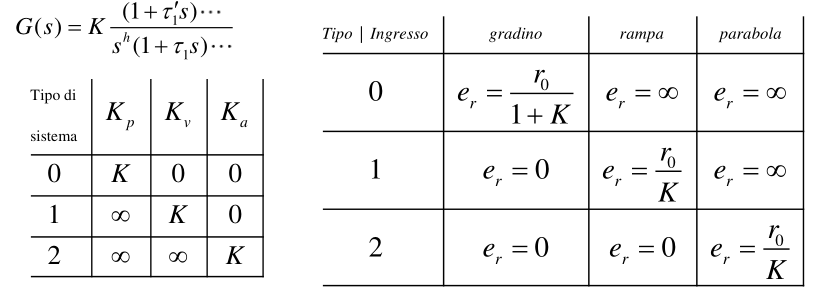
\includegraphics[width=0.5\linewidth]{./images/analisi_regime_retroazione.png}
  \caption{Analisi a regime dei sistemi in retroazione}
  \label{fig:analisi_regime_retroazione}
\end{figure}




\section{Sistemi retroazionati: criterio di Nyquist e margini di stabilità}

\subsection{Buona connessione}



\end{document}
